\documentclass[11pt,english]{article}
\usepackage[latin9]{inputenc}
\usepackage[letterpaper]{geometry}
\geometry{verbose,tmargin=1in,bmargin=1in,lmargin=1in,rmargin=1in}
\usepackage{babel}
\usepackage{amsmath}
\usepackage{amssymb}
\usepackage{capt-of}
\usepackage{graphicx}
\usepackage[usenames,dvipsnames]{color}
\usepackage{latexsym}
\usepackage{xspace}
\usepackage{pdflscape}
\usepackage{placeins}
\usepackage[hyphens]{url}
\usepackage[colorlinks]{hyperref}
\usepackage{enumerate}
\usepackage{ifthen}
\usepackage{float}
\usepackage{array}
\usepackage{tikz}
\usetikzlibrary{shapes}
\usepackage{algorithm2e}
\setcounter{MaxMatrixCols}{20}

\newcommand{\rthree}{\mathbb{R}^3}
\title{CIS 581 Homework 3 \\
}
 \author{Gabrielle Merritt}
 
\date{}

\begin{document}
\maketitle
\section*{ Seam Removal}
For seam removal I only removed one seam, but I used scatter plot to exaggerate the pixels I would be removing from the seam  
\begin{figure}[h]
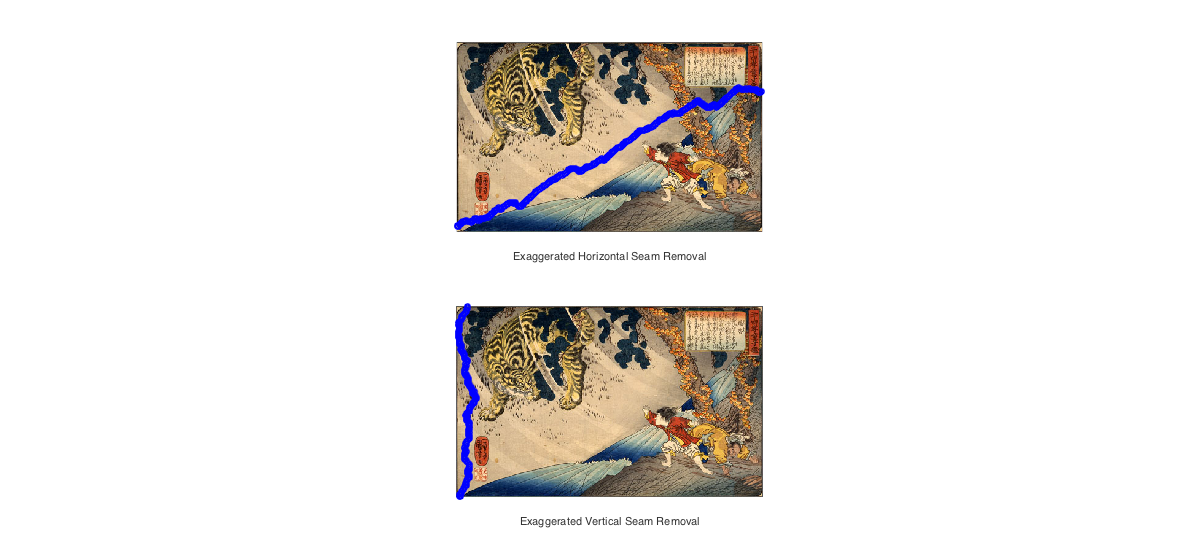
\includegraphics[width = \linewidth]{seam_removal}
\end{figure}

\section*{Mosaic}
For mosaic , I have a strong threshold on anms to keep it from running for a very long time. This method works for the Philadelphia Museum of Art stitch because it has very distinctive features. 

\subsection*{Feature Matching}
For mosaic , I have a strong threshold on anms to keep it from running for a very long time. This method works for the Philadelphia Museum of Art stitch because it has very distinctive features
\\
Yellow Circles are my adaptive non max suppression points (only using 50) 
\begin{figure}[h]
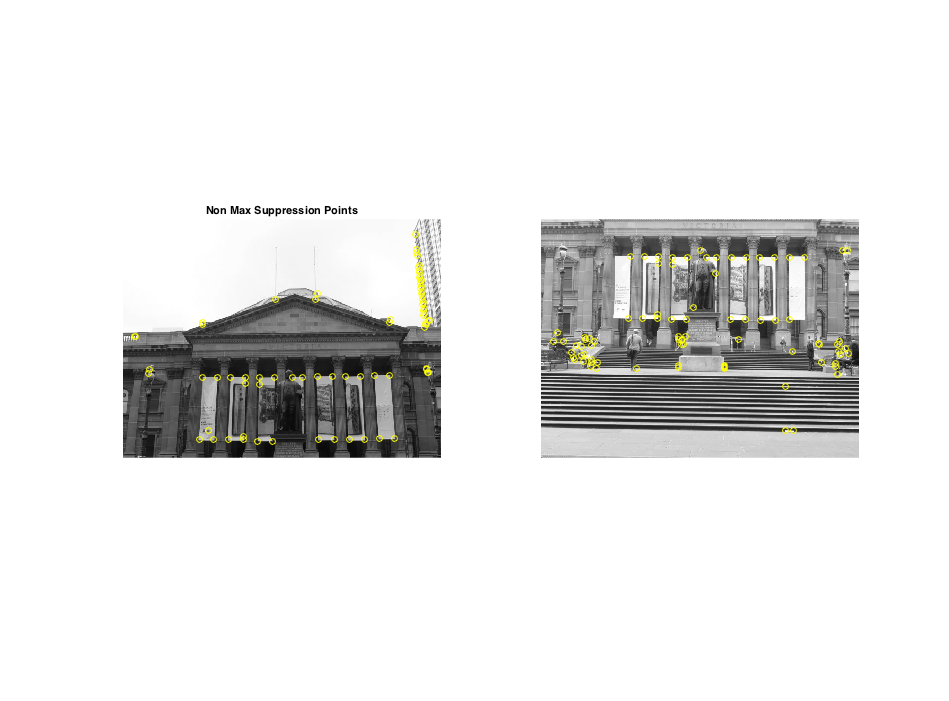
\includegraphics[width = \linewidth]{anms_pts}
\end{figure}
Red circles indicate post RANSAC matched features 
\begin{figure}[h]
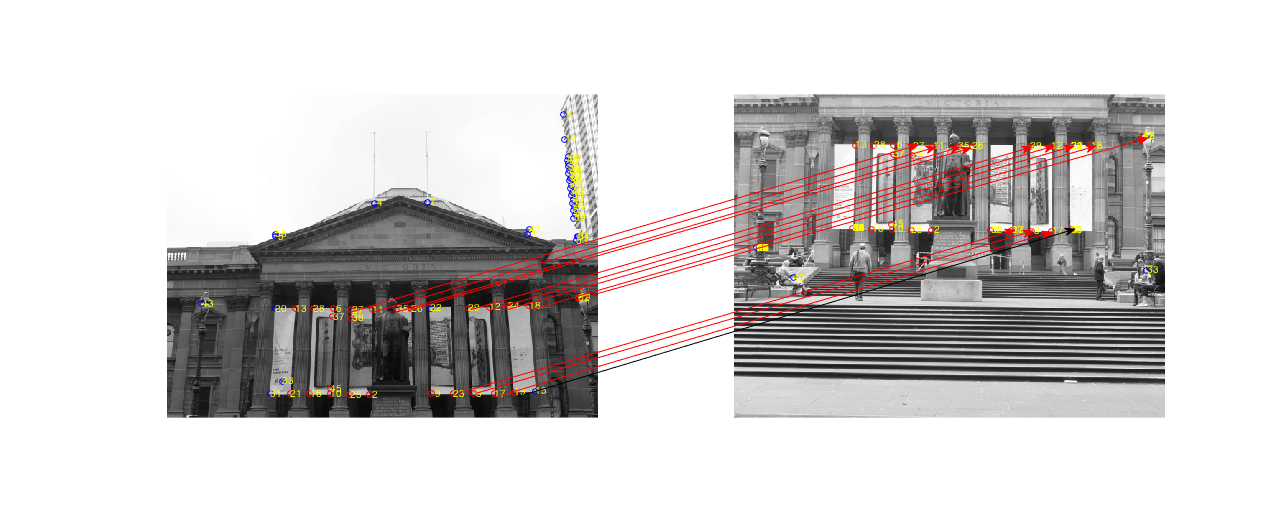
\includegraphics[width = \linewidth]{feature_matching_pma}
 \caption{Feature matching between middle Image another image}
\end{figure} 
\begin{figure}[h]
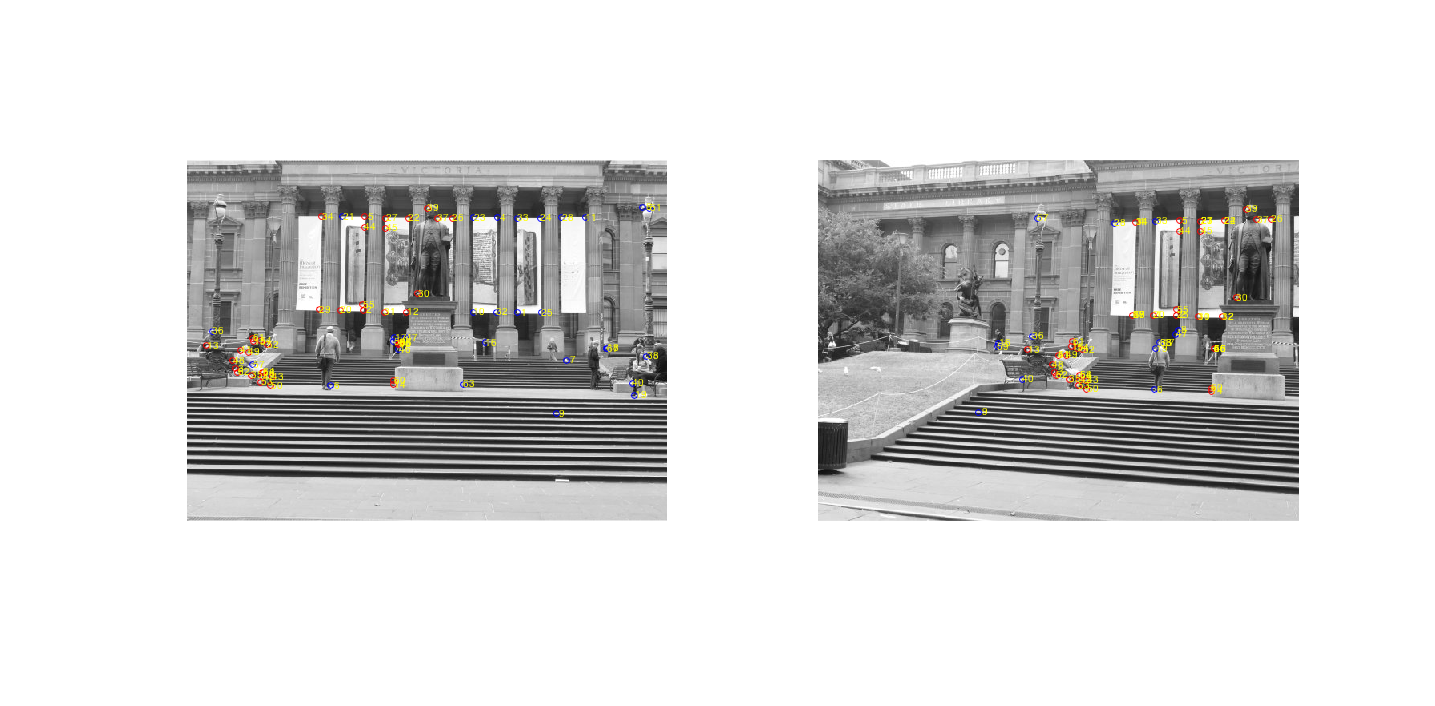
\includegraphics[width = \linewidth]{feature_matching_pma2}
\caption{ Red dots indicate ransac matched features}
\end{figure} 
\FloatBarrier 
\subsection*{Final Stitch }
Initially when I tried stitching I would stitch two images together, and then stitch another new image to this combined image, but because my blending was not good (even the vision tool box blending didn't help), my stitched images ended up giving many false edges, which fooled my featuring matching. \\
I relied heaviliy on matlabs example for panorama stitching for my mosaic, which lead to much better results, and fixed my feature matching issues.
\\
For the script I have now I find the middle picture by finding all of the transforms from first to last image and transforming the image extents, which ever image is closest to the middle of the transform of all the pictures I consider the middle image. Then repeat the process but multiplying all the homographies by the inverse of homography of the middle picture.\\
By stitching everything together at the end, I was able to get the full extents of the picture. 
\begin{figure}[h]
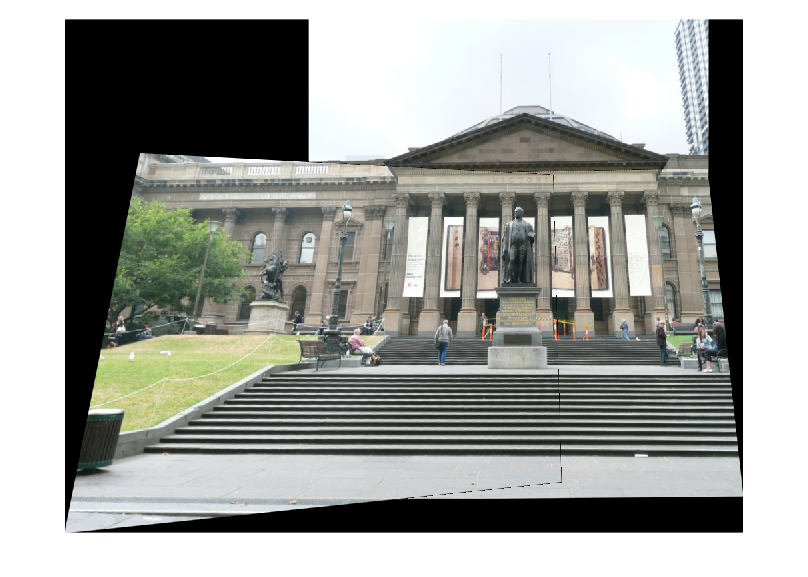
\includegraphics[width = \linewidth]{art_museum}
\end{figure}
\end{document}
